\documentclass[11pt]{article}
\usepackage{amsmath}
\usepackage{amssymb}
\usepackage{bm}
\usepackage{enumerate}
% \usepackage{fancyvrb}
\usepackage[top=1in, bottom=1in, left=1in, right=1in]{geometry}
\usepackage{hyperref}
\hypersetup{
    colorlinks=true,
}
\usepackage{multirow}
\usepackage{bbm}
\usepackage{color}
\usepackage{enumitem}
\usepackage{xcolor}
\usepackage{float}
\usepackage{subcaption}
\usepackage{graphicx}
\usepackage{tikz}

\usepackage{caption}
\DeclareCaptionFont{blue}{\color{LightSteelBlue3}}
\newcommand{\foo}{\color{LightSteelBlue3}\makebox[0pt]{\textbullet}\hskip-0.5pt\vrule width 1pt\hspace{\labelsep}}

\DeclareMathOperator*{\argmin}{arg\,min}
\DeclareMathOperator*{\argmax}{arg\,max}

\def\checkmark{\tikz\fill[scale=0.4](0,.35) -- (.25,0) -- (1,.7) -- (.25,.15) -- cycle;} 

\date{May 9, 2018}
\title{
11-797: Question Answering \\
Final Report \\[15pt]
Team: The Flying Riddlers 
}

\author{
    Vasu Sharma,
    Nitish Kulkarni, 
    Srividya Pranavi Potharaju,
    Gabriel Bayomi \\
    \texttt{[vasus, nitishkk, spothara, gbk, ehn, teruko] @cs.cmu.edu} \\
    Language Technologies Institute \\
    Carnegie Mellon University \\
}

\begin{document}
\maketitle


% \begin{abstract}
% In this paper, we present a novel Biomedical Question Answering system, \textit{BioAMA}: ``Biomedical Ask Me Anything" on task 5b of the annual BioASQ challenge \cite{bioasq}. In this work, we focus on a wide variety of question types including factoid, list based, summary and yes/no type questions that generate both exact and well-formed `ideal' answers. For summary-type questions, we combine effective IR-based techniques for retrieval and diversification of relevant snippets for a question to create an end-to-end system which achieves a ROUGE-2 score of 0.72 and a ROUGE-SU4 score of 0.71 on ideal answer questions (7\%  improvement over the previous best model). Additionally, we propose a novel NLI-based framework to answer the yes/no questions. To train the NLI model, we also devise a transfer-learning technique by cross-domain projection of word embeddings. Finally, we present a two-stage approach to address the factoid and list type questions by first generating a candidate set using NER taggers and ranking them using both supervised or unsupervised techniques.

% \end{abstract}

\section{Introduction}

% In the era of ever advancing medical sciences and the age of the internet, a remarkable amount of medical literature is constantly being posted online. This has led to a need for an effective retrieval and indexing system which can allow us to extract meaningful information from these vast knowledge sources. One of the most effective and natural ways to leverage this huge amount of data in real life is to build a Question Answering system which will allow us to directly query this data and extract meaningful and structured information in a human readable form. 

In the last few years, there have been tremendous advancements in the field of Question Answering, with the neural Question Answering systems outperforming even humans in some cases[\cite{msmarco}]. However, there is also a large diversity in the type and nature of existing QA systems, and most systems are very specific to a certain dataset. For a new QA dataset, it is still hard to predict what kind of QA models would be most befitting and the extent to which a QA model trained on one dataset would work on another. To that end, we present a comprehensive investigation into different types of QA systems based on question and answer types, as well as carefully analyze the relative merits and demerits of having a modularized question-type based system as opposed to an end-to-end QA system. 

\subsection{General Hypothesis}

With the key idea to assess the generalizability of a Question Answering system, we formulate our general hypothesis as: \\

For the task of Question Answering (QA), a comprehensive and holistic system can be designed that can handle multiple question/answer types and can yield a good performance across a number of QA datasets.

\subsection{Scope}

In order to test our hypothesis, we design and implement broadly two types of Question Answering systems - 1) a modularised question-type specific system and 2) an end-to-end system. We test the performance of these systems on two different datasets (one small and one large) in order to identify a general pattern of relative performances. 

We confine the scope of this work to the question types - yes/no, factoid, list, summary and description. We also consider fixed-sized manually-curated datasets in order to build supervised QA systems. The key focus of our work is, as mentioned earlier, to compare the relative performances of the two systems across different datasets and it is not to develop a single system that works best on a specific dataset. That being said, we do employ several techniques to improve the individual performances of both the systems in order to ensure a fair comparison.

% In this paper, we present  an end-to-end question answering system designed to handle the large variety of question types present in the BioASQ dataset which we call as ``\textit{BioAMA}: Biomedical Ask Me Anything".   \\

    %\item \textbf{Incorporating Information retrieval in the Question Answering pipeline}:
    %We incorporate Indri and BM25 based features in our pipeline to allow for effective information retrieval from the biomedical knowledgebase which allows us to choose the snippets which are most relevant to a given question. 
    %\item \textbf{Statistical ranking models}: We use the powerful LeTOR framework to allow for ranking of our snippets chosen by the information retrieval mechanism. This allows us to maximize the information we extract from the snippets which are deemed more relevant to a specific question. This also blends in well with our MMR framework which makes use of the ranking framework to extract the most relevant and non-repetitive information from the chosen snippets.
    
    %The rest of the paper is organized as follows. Section \ref{lit} presents the prior work on this problem followed by details of the BioASQ challenge and dataset in Section \ref{Dataset}. We present our approach and results for the ideal answer type questions in Section \ref{approach1} and for the exact answer type generation in Section \ref{approach2}. Finally we present the conclusions and future directions of our work in Section \ref{future}.


\section{Relevant Literature}
\label{lit}

The Question Answering problem is immensely popular among NLP researchers and large industrial research labs all over the world. The release of the SquAD data set \cite{squad} boosted this interest as many researchers began to use this data set to evaluate their approaches. However, the SquAD data set is only used to evaluate extractive question-answering systems and hence doesn't allow for free-form answers. The state of the art model for this problem presently is the Dynamic Co-Attention Network (DCN) from Xiong et al.  \cite{DCN}, the ensemble model of which presently holds the top spot on the SquAD leader board. The DCN first fuses co-dependent representations of the question and the document in order to focus on relevant parts of both. Then a dynamic pointing decoder iterates over potential answer spans. This iterative procedure enables the model to recover from initial local maxima corresponding to incorrect answers. \\

Other prominent works include the R-Net networks from Microsoft Research Asia \cite{Rnet} who introduce self matching networks to tackle this problem. They first match the question and passage with gated attention-based recurrent networks to obtain the question-aware passage representation. Then they propose a self-matching attention mechanism to refine the representation by matching the passage against itself, which effectively encodes information from the whole passage. Finally they employ the pointer networks to locate the positions of answers from the passages.\\

The Bidaf network from Seo et al \cite{bidaf} was one of the first landmark papers to demonstrate the effectiveness of attention based bidirectional recurrent networks on the task of Machine Comprehension.  They introduced a multi-stage hierarchical process that represents the context at different levels of granularity and uses bi-directional attention flow mechanism to obtain a query-aware context representation without early summarization. Many subsequent works on the problem now build on top of the Bidaf network.\cite{Sedt} from CMU and \cite{Reasonet} for Microsoft Research Redmond are some of the other prominent works on this problem. In \cite{Sedt} the authors encode the information from syntactic trees into the vector embeddings and use this added structured syntactic knowledge to improve their results on this task. In \cite{Reasonet}, the authors propose a reinforcement learning based approach to determine how many passes should the network make over the knowledge base during answer generation thereby doing away with restriction of fixed number of passes over the knowledge base.\\

Biomedical Question answering has always been a hot topic of research among the QA community at large due to the relative significance of the problem and the challenge of dealing with a non standard vocabulary and vast knowledge sources. The BioASQ challenge has seen large scale participation from research groups across the world. One of the most prominent among such works is from Chandu et al. \shortcite{khyati-paper} who experiment with different biomedical ontologies, agglomerative clustering, Maximum Marginal Relevance (MMR) and sentence compression. However, they only address the ideal answer generation with their model. Peng et al. \shortcite{fudan} in their BioASQ submission use a 3 step pipeline for generating the exact answers for the various question types. The first step is question analysis where they subdivide each question type into finer categories and classify each question into these subcategories using a rule based system. They then perform candidate answer generation using POS taggers and use a word frequency-based approach to rank the candidate entities. Wiese et al. \shortcite{fastqa} propose a neural QA based approach to answer the factoid and list type questions where they use FastQA: a machine comprehension based model \cite{fastqa-squad} and pre-train it on the SquaD dataset \cite{squad} and then finetune it on the BioASQ dataset. They report state of the art results on the Factoid and List type questions on the BioASQ dataset. Another prominent work is from Sarrouti and Alaoui \shortcite{usmba} who handle the generation of the exact answer type questions. They use a sentiment analysis based approach to answer the yes/no type questions making use of SentiWordNet for the same. For the factoid and list type questions they use UMLS metathesaurus and term frequency metric for extracting the exact answers. \\ %They also use the BM25 model and UMLS concepts for retrieving the ideal answers. \\

Despite the popularity of Machine Comprehension problems, very little work has been done on free-form answer generation for questions. The biggest reasons likely include the lack of large standard data sets, difficulty in evaluation and the inherent difficulty of `human-like' natural language generation. One of the only existing data sets for this problem is the MS Marco dataset released by Microsoft \cite{msmarco}. The top positions on this leader board are held by modifications of the RNet \cite{Rnet} and Reasonet \cite{Reasonet} algorithms. Most of these approaches generate the answer by using an attention based bidirectional LSTM network to generate the answer word-by-word conditioned on the knowledge base, question and the best answer span. However, most of these answers lack syntactic coherence, retention of long term dependencies and human-like answer quality, which have been the primary problems with free-form natural language generation. Here we explore approaches to try and solve these problems and try to improve the performance on Machine Comprehension and free-form response generation.\\


\section{Dataset}

We build our QA systems on two datasets: BioASQ dataset (from PubMed documents) and MAchine Reading COmprehension (MS MARCO) dataset (from web documents).

\subsection{BioASQ}
\label{Dataset}

BioASQ dataset is 
BioASQ challenge \cite{bioasq} is a large scale biomedical question answering and semantic indexing challenge, which has been running as an annual competition since 2013. %This challenge assesses the ability of systems to semantically index very large numbers of biomedical scientific articles, and to return concise and user-understandable answers to given natural language questions by combining information from biomedical articles and ontologies.
We deal with the Phase B of the challenge which deals with large scale biomedical question answering. The dataset provides a set of questions and snippets from PubMed, which are relevant to the specific question. It also provides users with a question type and urls of the relevant PubMed articles itself. The 5b version of this dataset consists of 1,799 questions in 3 distinct categories:
\begin{enumerate}
    \item \textbf{Factoid type}: This question type has a single entity as the ground truth answer and expects the systems to output a set of  entities ordered by relevance; systems are evaluated using the mean reciprocal rank \cite{MRR} of the answer entities with reference to the ground truth answer entity.
    \item \textbf{List type}: This answer type expects the system to return an unordered list of entities as answer and evaluates them using a F-score based metric against a list of reference answer entities which can vary in number.
    \item \textbf{Yes/No type}: This question type asks the systems to answer a given question with a binary output namely yes or no. The questions typically require reasoning and inference over the evidence snippets to be able to answer the questions correctly.
\end{enumerate}

The dataset expected the participants to generate two types of answers, namely, exact and ideal answers. 
In ideal answers, the systems are expected to generate a well formed paragraph for each of the question types which explains the answer to the question. They call these answers `ideal' because it is what a human would expect as an answer by a peer biomedical scientist. In the exact answers the systems are expected to generate ``yes" or ``no" in the case of yes/no questions, named entities in the case of factoid questions and list of named entities in the case of list questions.

\subsection{MS MARCO}

\section{Question-type based QA system} \label{approach2}

We now present a QA system which is a combination of several modules, each built to handle a specific question type. The reason we believe that such a system would be effective is because of that, in this case, the nuances of each of the question types can be appropriately captured in the modules and the modifications to one module to address its corresponding inadequacies will not affect the performance of any other. 
We build this system for the BioASQ dataset, primarily because of the unique challenges that the BioASQ dataset which call for a modularized system. 

In the sections that follow, we shall present the modules for handling the question types: yes/no, factoid/list and summary type. In addition to addressing each question type specifically, we also cater to different answer types: exact and ideal. Exact answers represent the subset of the BioASQ task where the responses are not structured paragraphs, but instead either a single entity (\textit{yes/no} types) or a combination of named entities (\textit{factoid} or \textit{list} types) that compose the correct reply to the given query. The main idea refers to evaluating if a response is able to capture the most important components of an answer. For factoid or list types of questions, we must return a list of the most likely entities to compose the answer. The main difference between them is that ground truth for \textit{factoid} questions is composed of only one correct answer and the evaluation method is Mean Reciprocal Rank (MRR). However, the ground truth for \textit{list} is an actual list of correct answers with varying length, which uses F-measure as an evaluation metric. The BioASQ submission format allows everyone to submit 5 ranked answers for \textit{factoid} and 1 to 10 answers for \textit{list}. For \textit{yes/no} questions, the ground truth is simply the yes or no label, using F-measure as an evaluation metric.

\subsection{Yes/No Type Questions}

Although yes/no questions require a simple binary response, calculating yes/no responses for the BioASQ question can be challenging: 
\begin{enumerate}
    \item There is an inherent class-bias towards the questions answered by \texttt{yes} in the dataset;
    \item The dataset is quite small for training a complex semantic classifier;
    \item An effective model must perform  reasoning and inference using the limited information it has available, which is extremely difficult even for non-expert humans.
\end{enumerate}

Due to the nature of the question type, these questions can not be simply classified by using word-level features. Learning the semantic relationship between the question and the sentences in the documents is quite elemental to solving this task. Hence, we present a Natural Language Inference (NLI)-based system that learns if the assertions made by the questions are true in the context of the documents. As a part of this system, we first generate assertions from questions and evaluate the entailment or contradiction of these assertions using a Recognizing Textual Entailment (RTE) model. We then use these entailment scores for all the sentences in the snippets or documents to heuristically evaluate if the answer to the yes/no question.

% \begin{figure}
%     \centering
%     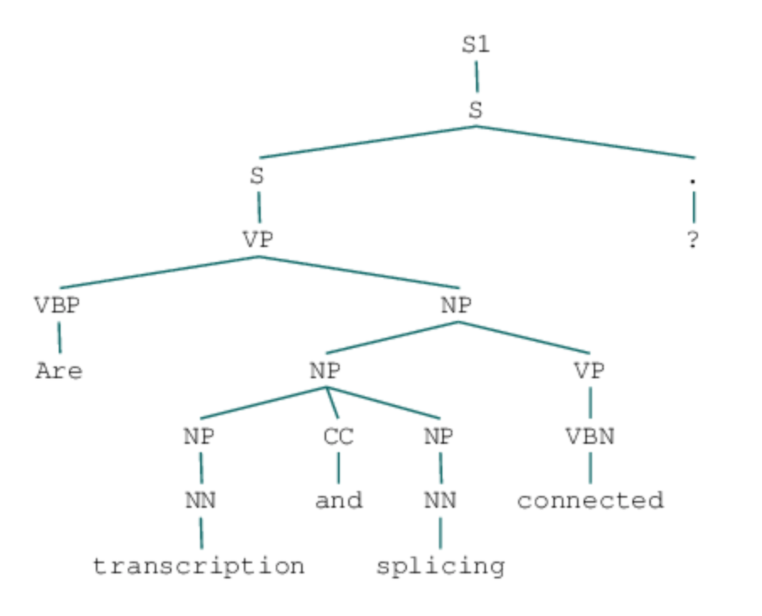
\includegraphics[scale=0.3]{images/question_parse.png}
%     \caption{The parse tree of an example question as generated by the BLLIP parser}
%     \label{fig:parse_tree}
% \end{figure}

\subsubsection{Assertion Extraction}

The first step towards answering the question is to identify the assertions made by the question. For this, we use a statistical natural language parser to identify the syntactical structure in the question. We, then, heuristically generate assertions from the questions.\\
Consider the following example question:

\textit{Is the monoclonal antibody Trastuzumab (Herceptin) of potential use in the treatment of prostate cancer?}

Upon parsing of this question, we have the phase constituents of the question. Almost all yes/no questions have a standard format that begins with an auxiliary verb followed by a noun phrase. In this example, we can toggle the question word with the first noun phrase to generate the assertion:

\textit{The monoclonal antibody Trastuzumab (Herceptin) is of potential use in the treatment of prostate cancer.}

In a similar manner, we then create positive assertions for all \textit{yes/no} questions as depicted in Figure . As a simple extension to this, we can also create negative assertions by using \textit{not} along with the auxiliary verbs.

\begin{table*}[t!]
    \centering
    \begin{tabular}{r l} \hline
        Question & Assertion \\ \hline
    \textit{Is} the protein Papilin secreted? & The protein Papilin \textit{is} secreted \\
    \textit{Are} long non coding RNAs spliced? & 
    long non coding RNAs \textit{are} spliced \\
    \textit{Are} transcription and splicing connected? &
    Transcription and splicing \textit{are} connected. \\
    \textit{Is} RANKL secreted from the cells? &
    RANKL \textit{is} secreted from the cells. \\
    \textit{Does} metformin interfere thyroxine absorption? & 
    Metformin \textit{does} interfere thyroxine absorption. \\
    \textit{Has} Denosumab (Prolia) been approved by FDA? &
    Denosumab (Prolia) \textit{has} been approved by FDA. \\
    % \textit{Is} Alu hypomethylation associated with breast cancer? & 
    % Alu hypomethylation \textit{is} associated with breast cancer  \\
    \hline
   \end{tabular}
    \caption{Assertion generation for some questions from training set in BioASQ Phase 6b by heuristic-based rearrangement of the auxiliary verb the questions starts with.}    \label{tab:assertion_examples}
\end{table*}

\subsubsection{Recognizing Textual Entailment}

The primary goal of our NLI module is to infer if any of the sentences among the answer snippets entails or contradicts the assertion posed by the question. We segmented the answer snippets for each question to produce a set of assertion-sentence pairs. To then evaluate if these assertions can be inferred or refuted from the sentences, we built a Recognizing Textual Entailment (RTE) model using the \textit{InferSent} model \cite{Infersent}, which computes sentence embeddings for every sentence and has been shown to work well on NLI tasks. In training \textit{InferSent}, we experienced two major challenges:

\begin{enumerate}
    \item The number of assertion-sentence pairs in BioASQ is too few to train the textual entailment model effectively.
    \item The models that are pre-trained on SNLI \cite{snli}
    datasets use GLOVE \cite{glove} embeddings that cannot be used for biomedical corpora which have quite different characteristics and vocabulary compared to the corpora that GLOVE was trained on.
\end{enumerate}

However, we have pre-trained embeddings available that were trained on PubMed and PMC texts along with Wikipedia articles \cite{biomed_embed}. To leverage these embeddings, we implemented an embedding-transformation methodology to projecting the PubMed embeddings to GLOVE embedding space and then fine tune the pre-trained \textit{InferSent} on the BioASQ dataset for textual entailment. The hypothesis is that, since both the embeddings had a significant fraction of documents in common (Wikipedia corpus), by transforming the embeddings from one space to another, the sentence embeddings from the model would still represent a lot of the semantic features of the input sentences that can subsequently used for classifying textual entailment. For this task, we explore both linear and non-linear methods of embedding transformation.

While simple, a linear projection of embeddings from one space to another has shown to be quite effective for a lot of multi-domain tasks. By imposing an orthogonality constraint on the project matrix, we model this problem as an orthogonal Procrustes problem: \\
Let $d_p$ and $d_g$ be the embedding dimensions of PubMed embeddings and GLOVE embeddings respectively.
If $E_p$ and $E_g$ are the matrices of PubMed embeddings ($N \times d_p$) and their corresponding GLOVE embeddings ($N \times d_g$) for the words that both the embeddings have in common ($N$), the projection matrix ($d_g \times d_p$) can be computed as,
\begin{align*}
    W^* &= \argmin_W \lVert  W E_p^{\intercal} - E_g^{\intercal} \rVert
\end{align*}
subject to the constraint that $W$ is orthogonal.
The solution to this optimization problem is given by using the singular value decomposition of $E_g^{\intercal} E_p$, i.e.$  W^* = UV^{\intercal}$ where $E_g^{\intercal} E_p = U \Sigma V^{\intercal}$
With this simple linear transformation, we then computed the transformed embeddings for all the words in the PubMed embeddings that are not present in the GLOVE embeddings. 

We also explore a non-linear transformation using a feed-forward neural network where the the objective is to learn function $f$ such that, $f(e_p; \theta) = e_g$ where, $e_p$ and $e_g$ are PubMed and GLOVE embeddings respectively. We model $f$ using a deep neural network with parameters $\theta$, and train using the common words in both the embeddings. 
% The effectiveness of this training is a result of the large number of common vocabulary between the two embeddings (since both are trained on Wikipedia text among other corpora).

%\end{enumerate}

The transformed embeddings from these models were used in conjunction with the pre-trained \textit{InferSent} model to encode the semantic features of the biomedical sentences as sentence embeddings. Subsequently, we employ these sentence embeddings of the assertion-sentence pairs for a particular question to train a three-way neural classifier to predict if the relationship between the two is entailment, contradiction or neither. 

It is worth noting here that the embedding transformation techniques that we implemented are not specific to the NLI tasks and, in fact, enable transfer learning of a much broader set of tasks on smaller datasets like BioASQ by using the pre-trained models on large datasets of other domains and fine-tuning on the smaller dataset.

\subsubsection{Classification}

As a final step, we use the textual entailment results for each assertion-sentence pair generated to heuristically classify the answer as \textit{yes} or \textit{no}. Since our system comprises multiple stages with the errors of each cascading to the final stage, we do not get perfect entailment results for the pairs. However, since we have a lot of pairs, we aggregate these entailment scores to compute the overall entailment or contraction scores to reduce the effect of accumulated errors for individual pairs on classification.

We used a simple unsupervised approach for classification by just comparing the overall entailment and contradiction scores, i.e. if the total number of snippet sentences that entail the assertion are $N_e$ and the total number of snippet sentences that contradict are $N_c$, then, 
\begin{align*}
    \text{answer}_{\text{q}} = \begin{cases}
    \text{yes} & \text{if } N_e \ge N_c \\
    \text{no} & \text{ otherwise}
    \end{cases}
\end{align*}

\begin{figure*}[t!]
    \centering
    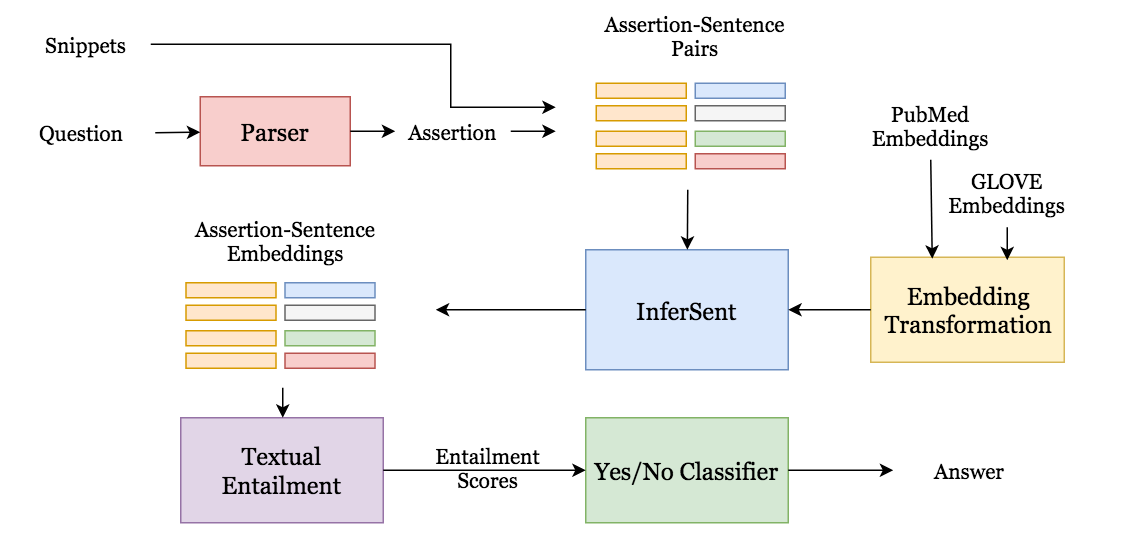
\includegraphics[width=0.95\textwidth]{images/YesNoPipeline.png}
    \caption{The complete system for yes/no answer classification using a question and relevant snippets}
    \label{fig:yesno_pipeline}
\end{figure*}

The end-to-end architecture of our system from the input questions and snippets to the answer is shown Figure \ref{fig:yesno_pipeline}.

\subsubsection{Experimental Details}

For parsing the questions, we used BLLIP reranking parser \cite{charniak_new1} (Charniak-Johnson parser) %\cite{charniak_new1} 
and used the model \texttt{GENIA+PubMed} for biomedical text. For training the textual entailment classifier using \textit{InferSent}'s sentence embeddings, we used Stanford's SNLI \& Multi-NLI dataset \cite{snli} to achieve a test-set accuracy of $84.7 \%$.
%TODO: Specify details for non-linear embedding transformation

\subsubsection{Results}

The performance of the system on yes/no questions on the training set of phase 5b has been tabulated in table \ref{tab:yesno_results}. While the accuracies are better than a random classifier, the task is far from being solved. Nonetheless, the classifier does handle the class bias in the training data and performance similarly on both the categories of answers. Moreover, this classifier achieved the second best test accuracy of 65.6\% on phase 5 of BioASQ 5b (Table \ref{tab:comparison_results}). While we implemented a simple heuristic based answer-classifier, we believe that a supervised classifier using the sentence embeddings as well as fine-tuning of the textual entailment classifier on BioASQ dataset would considerably enhance the overall performance of the system.

\begin{table}[t!]
    \centering
    \begin{tabular}{c|l} \hline
    
    Category & Accuracy (\%) \\ \hline
    Yes      &  56.5  (252/444)\\
    No       &  58.9 (33/56) \\
    Overall  &  57.0 (285/500) \\      \hline
    \end{tabular}
    \caption{Class-wise accuracies on yes/no questions in training set of BioASQ Phase 5b}
    \label{tab:yesno_results}
\end{table}


\subsection{Factoid \& List Type Questions}

% The key objective in extraction-based factoid and list type question answering systems is to find a subset of entities (or phrases) from the relevant snippets that are most likely to answer the question. 
Most of the state-of-the-art models for this task involve training end-to-end deep neural architectures to identify a subset of entities (or phrases) from the relevant snippets that are most likely to answer the question. But, owing to the small size of the dataset, we cannot effectively train such models on the BioASQ dataset. Hence, we adopted a two-stage approach that first finds a set  of entities that could potentially answer the question and a supervised classifier to rank the entities on the basis of their likelihood of answering the question.

For devising the model and evaluation, we primarily focused on factoid type questions since the methodology for the list-type question would be largely similar and different only in the number of top entities returned. 


\begin{table}[h]
    \centering
    \begin{tabular}{cccc} \hline
    \multirow{3}{*}{NER Tags} & 
    \multicolumn{2}{c}{\% of questions} & 
     \% of \\
    & Exactly & Partially & tokens \\
    & Answered & Answered & extracted \\ \hline
    PubTator & 32.05 &	72.15 & 52.27 \\
    Gram CNN & 34.90 &	99.03 & 94.97 \\
    LingPipe & 26.67 &	76.75 & 11.06 \\
    Union    & 49.04 &	99.65 & 99.25 \\
    Intersection & 16.29 &	38.00 & 3.33 \\ \hline
    \end{tabular}
    \caption{Baseline recall of different NER Taggers measured by the fraction of questions that can be answered by an ideal classifier if the candidates are chosen using the tagger. We also measure precision as the fraction of total unique tokens from the documents that are tagged.}
    \label{tab:NER_tagging_performances}
\end{table}

\begin{table*}[t!]
    \centering
    \begin{tabular}{|c|c|c|c|c|} 
    \hline \hline
    Model & Exact Answers & Exact Answers & Exact Answers & Ideal Answers \\
    &Yes/No type& Factoid  type& List type & All types \\
    & Accuracy (\%) & MRR & F1 score & ROUGE-2\\
    \hline \hline
    \cite{khyati-paper} & - & - & - & 0.653  \\
    \hline
    \cite{fudan}&\textbf{0.714}&0.272& 0.187& -\\
    \hline
    \cite{fastqa}& - &\textbf{0.392}& \textbf{0.361}&-\\
    \hline
    Sarrouti and Alaoui \shortcite{usmba}&0.461&0.207&0.243&0.577\\
    \hline
    \textit{BioAMA}(Ours)&0.653& 0.195&0.234&\textbf{0.721}\\
    \hline \hline
    
    \end{tabular}
    \caption{Comparison of our model with other state of the art approaches}
    \label{tab:comparison_results}
\end{table*}
\vspace{-0.3cm}


\subsubsection{Initial Hypotheses}


dsasadsa

\subsubsection{Candidate Selection}

We found that the most critical step in the answer generation process is to identify the set of potential answer candidates that can be fed into a classifier or ranker to identify the best candidates. At first, in order to accomplish this, we used Named Entity Recognition (NER) taggers to form a set of candidate answers. The taggers that we used include Gram-CNN \cite{gram-cnn}, LingPipe\cite{lingpipe} and PubTator \cite{pubtator}. To analyze the effectiveness of these taggers, we performed an analysis on BioASQ training set 5b by evaluating the fraction of questions whose answers are included in the candidate entity set by the taggers.

Table \ref{tab:NER_tagging_performances} shows the relative performances of the three taggers, their union as well as intersection on train dataset of BioASQ 5b factoid type questions. A question is exactly answered if a tagger tags an entity that matches an answer exactly, and it is partially answered if there is a non-zero overlap with an entity tagged and an answer for the question. We can notice that PubTator and LingPipe have a good recall with relatively low precision, while Gram CNN has high recall but low precision. However, the final results with the Named Entity Taggers were not aligned with our expectations. This is mostly because the answers for BioASQ are usually a combination of BioNERs and complementary words, making it hard to define a pruning method that is able to yield satisfactory results. Surprisingly, a group of candidates formed of the 100 most frequent \texti{n}-grams (\textit{n} from 1 to 4) from the snippets' sentences were a better candidate group than the NER approach for our supervised ranking method and we decided to use the NER taggers as features instead of candidate groups.


\subsubsection{Classification Features}\label{sec:classification_features}

Upon computing the set of candidate answers, we use the question $q$, set of relevant snippet sentences $\mathcal{S}$ and entity type $t_i$ to devise a feature vector for each individual entity $e_i$ that comprises the following features:

\begin{itemize}[noitemsep]
    \item BM25 Score: The BM25 scores for all the sentences are computed with the question as the query. Then, the scores of the sentence that contain the entity are aggregated to compute the BM25 score for the entity, i.e.
    \begin{align*}
    %     \text{BM25 }&\text{Score($e_i$)} \\
    %   &= \sum_{s \in \mathcal{S}} \text{BM25 Score($e_i$)} \cdot \mathbbm{1}(s, e_i)
        \text{Score}_{BM25}(e_i) &= \sum_{s \in \mathcal{S}} \text{Score}_{BM25}(e_i) \cdot \mathbbm{1}(s, e_i)
    \end{align*}
    where $\mathbbm{1}(s, e_i)$ is 1 iff sentence $s$ has entity $e_i$.
    \item Indri Score: Computed in the same manner as BM25 score in (i)
    \item Number of Sentences: Number of sentences $s \in \mathcal{S}$ that contain the entity $e_i$
    \item NER Tagger: A multinomial feature that represents which tagger among PubTator, LingPipe and GramCNN the entity was extracted with. This feature is included to identify the relative strengths of the different taggers.
    \item Tf Idf: The aggregate Tf-Idf scores of the entity with $\mathcal{S}$ as the set of documents
    \item Entity Type: Is a boolean feature that is 1 if the type of the entity (for example, \textit{gene}) is present in the question, and 0 otherwise.
    \item Relative Frequency: The amount of times the entity appears on the snippets' sentences divided by the total appearance of all of the relevant entities.
    \item Query Presence: Is a boolean feature that is 1 if the query contains the entity completely and 0 otherwise.

\end{itemize}

\subsubsection{Unsupervised Ranking}

As a baseline, we first present an unsupervised ranking system for the candidate answers. In this system, the snippet sentences are first ranked using the BM25 model. Then, for each entity, a score is computed by aggregating the BM25 scores of the sentences in which the entity is present. The rationale for this is that the entities in the top ranked sentences are more likely to be the answers. This entity score (which is equivalent to the BM25 score described in \ref{sec:classification_features}) is then used to rank the entities and return the top $k$ entities as answers to the question. The overall unsupervised system is shown in Figure \ref{fig:UnsupervisedNERPipeline}.

\begin{figure}
    \centering
    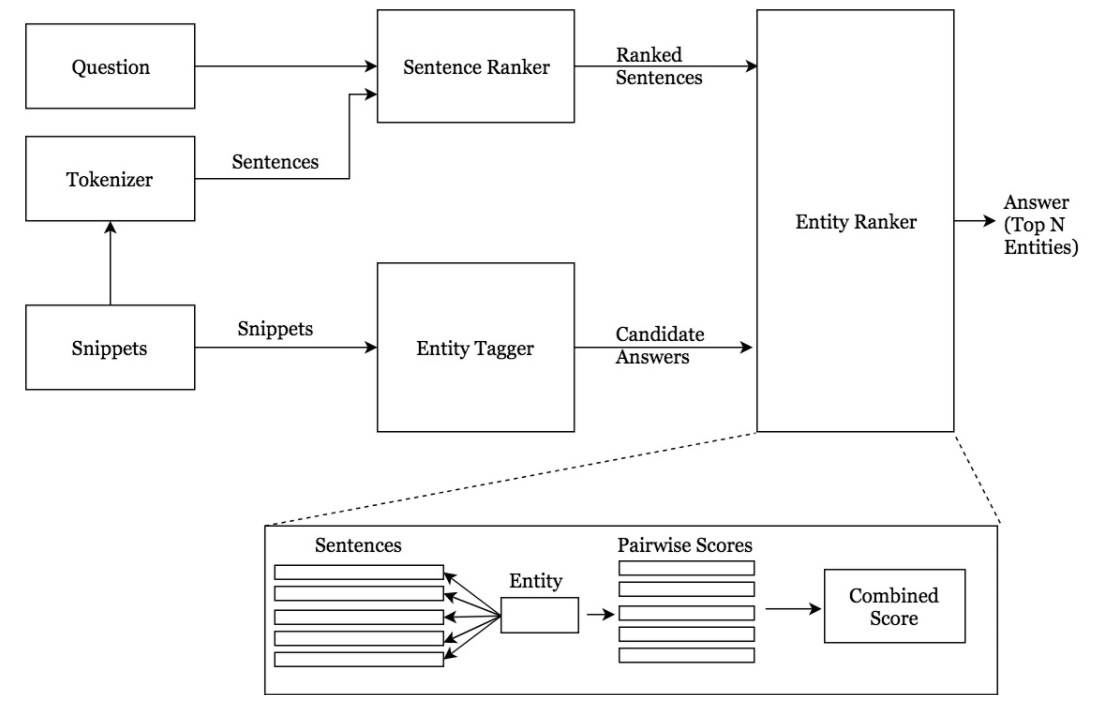
\includegraphics[scale=0.4]{images/UnsupervisedNERPipeline.png}
    \caption{Unsupervised generation of factoid/list type answers using NER taggers and BM25 retrieval model}
    \label{fig:UnsupervisedNERPipeline}
\end{figure}

\subsubsection{Learning To Rank}

In order to rank the candidate entities in a supervised way, we used a ranking classifier based on the features described in \ref{sec:classification_features}. For ranking, we chose point-wise ranking classifiers over pair-wise and list-wise, because it yields similar results to ranking methods with a less time-consuming and computationally expensive approach. We are using a traditional SVM-Light \cite{svmlight} implementation for point-wise ranking. The data for supervision was derived from the actual answers and candidate entities were ranked based on their overlap with the actual answers. 

% and the model was trained to learn these rankings.

% The idea behind our approach for factoid and list types of questions are based on pairwise Learning To Rank (LeToR). Each questions consists of a group of snippets and the actual query body. Given a Candidates Space (C) of possible named entities, a query (q) and a group of sentences extracted from the snippets (S); our approach is to train a model which ranks each candidate c of C given S and q. Basically, we are learning a function $g(c_i,c_k,S,q)$ that incorporates a score for each pair ($c_i,c_k$) of the Candidates Space. With the respective rankings, we can create a ranked list of entities to be returned. Therefore, in order to execute the model, it's necessary to define a Candidates Space C; a feature vector for each combination $f(c_i,S,q)$; and a function g for $g(c_i,c_k,S,q)$.

Once we rank the entities, we use a naive approach of merely taking top 5 entities as answers for factoid type and top 10 for list-type. One could, however, devise a separate model for identifying the number of top entities to return as answers for the list-type answers. 

We found that using just the NER entities as the answer candidates, the classifier could achieve an MRR of 0.06 on factoid type questions and an F-measure of 0.18 for list type questions. However, by having all the n-grams ($n = 1, 2, 3, 4$) from the snippets as candidate answers and using NER tags as LeToR features, the performance was improved to an MRR of 0.195 on Factoid type questions and an F1 score of 0.234  on List type questions. The results are summarized in Table \ref{tab:comparison_results}.


\subsubsection{Error Analysis}

\subsubsection{Hypotheses Confirmation/Revision}

% \newline \textbf{Features}: For features, we have used combination of syntactic, information retrieval, information theory, semantic and lexical features. POS tags, frequency, tf-idf, NER tags are examples of the features extracted for each candidate representation, which would consist of a vector of values between 0 and 1.  Therefore, for each candidate answer c for a question, we have a vector $v = f(c_i,S,q)$ that represents the features for this candidate.

% By directly testing and combining results, we decided to use the union of PubTator and LingPipe entities to build our Candidate Space. However, this was an insufficient approach due to the fact that it was too narrow to actually achieve reasonable results. Although the features chosen and the ranking model worked well, there was an upper bound precision available by this approach. Therefore, we shifted for different approaches: Noun's combinations, entity recognition systems not related to the biological domain and noun phrases. Noun Phrases have shown the best results: they are a large enough space (it doesn't create a hard bound limit for our results), but still possible to search and rank.

%\subsubsection{Results}
%The results of our list and factoid type questions are presented in Table \ref{tab:comparison_results}.

%\begin{table}[t!]
%    \centering
%    \begin{tabular}{ccc} \hline
%    Entities & Soft Accuracy (\%) & MRR (\%) \\ \hline
%    Pubtator & \textbf{7.14} & 3.35 \\
%    Lingpipe & 4.58 & 2.70 \\
%    Gram CNN & 0.98 & 0.24 \\
%    Union    & 1.05 & 0.38 \\
%    Intersection & 4.91 & \textbf{3.68} \\ \hline
%    \end{tabular}
%    \caption{Performance of unsupervised ranking model to identify the entities among the candidates from different taggers, for factoid type questions in BioASQ 5b dataset}
%    \label{tab:my_label}
%\end{table}

% Model	Exact Matches	Soft Matches	MRR Exact
% Pubtator	7.14%	50.71%	3.35%
% Lingpipe	4.58%	60.72%	2.70%
% Gram CNN	0.98%	85.53%	0.24%
% Ensemble Union	1.05%	85.29%	0.38%
% Ensemble Intersection	4.91%	39.47%	3.68%


\subsection{Summary Type Questions}
\label{approach1}
This section describes our efforts to address the ideal answer category on BioASQ along with the description type category of MS MARCO. % where the goal is to produce a query-based, relevant, non redundant and coherent summary answer from multiple snippets and documents. 
We proceeded with this answer type category with the specific hypothesis in mind. They are:
\begin{itemize}
\item Hypothesis 1: A QA system that provides accurate, non-repetitive answers must be supported by a strong Information Retrieval system.
\item Hypothesis 2: Human readability is a harder problem to tackle with. Abstractive methods perform better on this front than the extractive methods	\end{itemize}


 \begin{figure*}
     \centering
     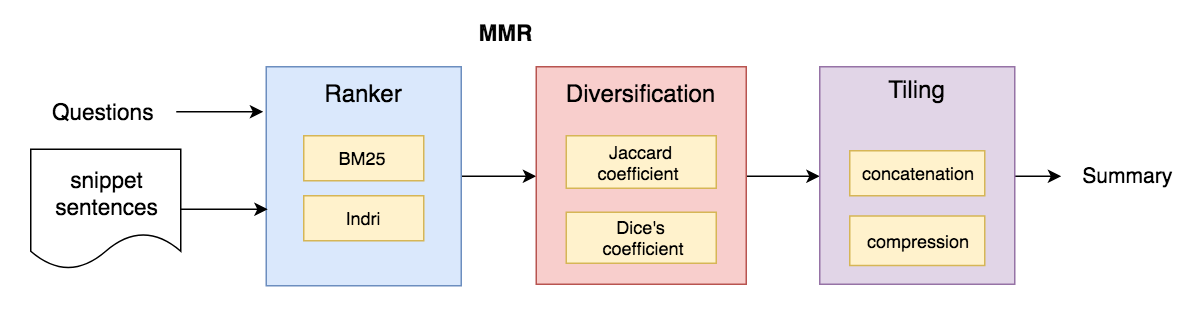
\includegraphics[scale=0.3]{images/pipeline_summary.png}
     \caption{Pipeline for ideal answer generation}
     \label{fig:ideal_answers_pipeline}
 \end{figure*}
\subsubsection{Extractive summarization}
Our pipeline for ideal answers has three stages. The first stage involves pre-processing of answer snippets and ranking of answer sentences by various retrieval models described in the following sections. The retrieval model scores form the soft positional component introduced in the MMR algorithm. We perform sentence selection next, where we select the top 10 best sentences for generating an ideal answer. The third and final stage involves tiling together the selected sentences to generate a coherent, non redundant, ideal answer for the given question. 
 %We describe our improvements to the pipeline that can be applied to all the above categories with primary focus being summary type questions as described in Section \ref{Dataset}.
The subsequent subsections explain the full pipeline for ideal answer type questions in detail (see Figure \ref{fig:ideal_answers_pipeline}).

\subsubsection{Question-Sentence Retrieval}
In this section we describe various approaches which were adapted to improve the initial retrieval of candidate sentences. We used the standard BM25 algorithm with custom pre-processing to exclude medical entities from stop word removal.  

\subsubsection*{BM25}
BM25 \cite{BM25} is a standard tf-idf based retrieval algorithm relying on bag of words approach for document retrieval. We considered every question to be independent and built an inverted index over the relevant snippets following the standard methods. Since the snippets are short paragraphs and the question is of moderate length, we tuned BM25 parameters accordingly. We customized the pre-processing by creating our own set of stop words that excluded certain bio-medical entities which might have been considered an English stop-word.

\[Score(D, Q) = \sum_1^n IDF(q_i) \frac{f(q_i, D) (k_1 + 1)}{f(q_i, D) + k_1 (1- b + b . \frac{|D|}{avgdl})} \]



\subsubsection*{Indri}

Indri \cite{Indri} is more modern retrieval model based on the use of statistical language models and query likelihood. We assumed a uniform prior over the sentences and ranked the candidate sentences based on the probability of the question given the sentence. 
We employed a two-stage smoothing that considers characteristics of both the query (the question in this context) and answer sentences. 

The Indri score for a candidate sentence is estimated in a collection (C) of snippets as follows:
\begin{align}
    & p(q_i|d) = (1-\lambda) p_{mle} (q_i|d) + \lambda p_{mle} (q_i|C) \label{eq1} \\ 
    & p_{mle}(q_i|d) = 
    \frac{tf + \mu  p_{mle}(q_i|C)}{length(d) + C} \label{eq2} \\ 
    & p_{mle}(q_i | C) = \frac{ctf}{length(C)}
\end{align}

where, $\lambda$ is the coefficient for linear interpolation based smoothing that accounts for question length smoothing. Since the questions are of moderate length, after tuning, the best value of $\lambda$ is attained at 0.75

In equation \ref{eq2}, $\mu$ is parameter for Bayesian smoothing using Dirichlet priors used for sentence length normalization. Since sentences of snippets can be of varying lengths, after tuning, the best value of $\mu$ is attained at 5000.

Both of the above smoothing techniques do two different things, the mixture model (interpolation) compensates for differences in the word importance (gives idf-effects) and the Dirichlet prior improves the estimates of the sentence sample which supports our decision to use two stage smoothing. 

% \subsubsection{LeToR}

% Learning to Rank \cite{Letor} is widely used, supervised learning approach for ranking the candidate sentences. We propose a new technique to create gold data for training the LeToR model. For every training data sample, we created a golden ranking of the sentences by ranking the candidate sentences from all the given snippets using golden ideal answer as the question following BM25 algorithm. For feature engineering part of LeToR, we considered different semantic, statistical and language model based features.
% \begin{itemize}
%     \item \textbf{Tf-Idf based}: BM25 score of the sentence
%     \item \textbf{Language model based}: Indri score of the sentence
%     \item \textbf{Semantic}: Count of the Named Entities in each sentence.
%     \item \textbf{Biomedical entities}: We obtained the biomedical entities from biomedical entity extraction tools like PubTator \cite{pubtator}, Lingpipe \cite{lingpipe} and GramCNN \cite{gramcnn}.
% \end{itemize}
% BM25, Indri algorithms were adapted as features for LeToR which was our final model for ranking candidate sentences


\subsection{Sentence Selection}
Once the top most relevant snippets have been chosen, we want to choose sentences from these snippets which are most relevant to a specific question. In this section we demonstrate how this selection is done.

\subsubsection{MMR}

We use the Maximum Marginal Relevance (MMR) algorithm \cite{MMR} as the baseline for sentence selection. In contrast to the basic Jaccard similarity metric used in previous work \cite{khyati-paper}, we experimented with other similarity measures which consistently perform better than the Jaccard baseline. MMR ensures the selected set contains non-redundant yet complete information. The sentences are selected based on two aspects, the sentence's relevance to the question and how different it is to the already selected sentences. At each step we select a document to append to the ranking based on the equation below.
\vspace{-0.3cm}
\begin{equation}
     d_i = \argmax_{d_j\in R \setminus S} (\lambda \cdot sim(q, d_i)  - (1 - \lambda) \cdot max\limits_{d \in \mathcal{S}}(sim_{sent}(d_i, d_j) ) ) \label{eq4}
\end{equation}
   

 We define a custom similarity metric between documents which uses positional values of sentences from the initial ranking as follows:
 \vspace{-0.3cm}
\begin{equation}
  sim_{sent}(di, dj) = ( 1 - \beta) \cdot (1 - \frac{rank(s_i)}{n}) + \beta \cdot sim(d_i, d_j) 
\end{equation}
Here, $sim_{sent}(di, dj)$ is the sentence to sentence similarity, $sim(q, di)$  is the question - sentence similarity, $rank(s_i)$ is the rank of the snippet which contains the sentence $d_i$, $S$ are Sentences already selected for summary i.e. which are ranked above this position. In the above equation, we tried various metrics to account for the sentence to sentence similarity. In cases where $\beta$ is non-zero, equation \ref{eq4} is identified as our SoftMMR which includes soft scoring based on sentence position.

\subsubsection{Dice's similarity Coefficient (DSC)}

Dice's similarity Coefficient (DSC) \cite{dice} is a quotient of similarity between two samples and ranges between 0 and 1 calculated as
It is used to compare similarity of two strings using bigrams. It is different from the Jaccard coefficient which counts intersecting words only once in both the numerator and denominator. 

\begin{equation*}
    dsc = \frac{(2 * n_t)}{ (n_x + n_y)}
\end{equation*}
where $n_t$ is the number of character bigrams found in both strings, $n_x$ is number of bigrams in string $x$ and $n_y$ is the number of bigrams in string $y$.
\subsection{\textbf{Evaluation}}
\subsubsection{BioASQ} 
The pipeline described above is primarily designed to improve the ROUGE evaluation metric \cite{Rougue}. Although a higher ROUGE score does not necessarily reflect improved human readability, MMR can improve readability by reducing redundancy in generated answers.
Results for ideal answers for Task 5 phase b for BioASQ dataset are shown in Table \ref{tab:rouge_extractive_summarization}. We also compare our results with other state of the art approaches in Table. Based on the results we accept our hypotheses 1 that a QA system needs to have strong IR  \ref{tab:comparison_results}.
\subsubsection{MS MARCO}
Now coming to the MS MARCO description dataset, the same pipeline couldn't be applied as is. Summary of BioASQ and Description of MS Marco are not exactly the same. Summary of BioASQ can be seen a subset of Description. The main difference being the average length of the description type answers. As mentioned in the dataset statistics, considering the number of sentences and average sentence length, we changed the number of words in summary from 200 to 20-25. That significantly improved our BLEU. Also, please note that we have performed the experiments on a smaller sample of the data. The results for description type questions are seen in the table \ref{tab:ms_marco_ext_res}.

\begin{table}[t!]
    \centering
    \begin{tabular}{|l|c|c|c|}
         \hline
            $\beta$& Configuration & Rouge-2 & Rouge-SU4 \\
        \hline
        \hline
        - & baseline & 0.7064 & 0.6962 \\
        \hline
        0.5 & BM25, Jaccard  & 0.7175 & 0.7110  \\ 
        \hline
        0.5 & BM25, Dice & 0.7193 & 0.7106  \\ 
        \hline
        0.6 & BM25, Dice & 0.7133 & 0.7053  \\ 
        \hline
        0.6 & BM25, Jaccard & 0.7133 & 0.7053  \\
        \hline
        \textbf{0.5} & \textbf{ Indri, Jaccard} & \textbf{0.7206} & \textbf{0.7135}  \\ 
        \hline
         0.5 & Indri, Dice & 0.7113 & 0.7052  \\ 
        \hline
    \end{tabular}
    \caption{ROUGE scores for different experiments on similarity metrics for extractive summarization}
    \label{tab:rouge_extractive_summarization}
\end{table}

\begin{table}[t]
    \centering
    \begin{tabular}{|c|c|c|c|c|} \hline
    \textbf{Configuration} & \textbf{Bleu 1} & \textbf{Bleu 2} & \textbf{Bleu 3} & \textbf{Rouge-L} \\
    \hline
      Wordlimit = 25, BM25, DuoSimilarity & 0.215 & 0.139 & 0.109 & 0.175\\
     \hline
     Wordlimit = 50, BM25, DuoSimilarity &  0.206 & 0.108 & 0.093 & 0.162\\
    \hline
    \end{tabular}
    \caption{Results on the MS Marco dataset}
    \label{tab:ms_marco_ext_res}
\end{table}

\subsubsection{Abstractive Summarization}
Neural sequence-to-sequence models have provided a viable new approach for abstractive text summarization insteas of simply selecting and rearranging passages/sentences from the original text. However, these models have a problem where the summary generated looks like sentences stitched together and not readable as if generated by a human.To address this, we tried Pointer Generator Networks as mentioned in \cite{PGC}

However, we couldn't get the expected results due to multiple reasons. We used a pretrained model which was trained on CNN daily mail data which lead to many UNKs (Unknown words) due to difference in the Vocabulary. Also we didn't add the coverage mechanism for penalizing repetitive sentences. This is a direction for our future work.

\subsubsection{Error Analysis}
\begin{itemize}
    \item Case 1: When the question asks to describe a very specific aspect/ affect. \\
    E.g.: \textit{What causes genetic alterations in normal cells ?}
    Here the question asks to narrow a specific reason that explains a scenario. The answer generated by the system spoke about genetic alterations in normal cells and its characteristics but not causes.
    \item Case 2: When the answer is beyond the understanding of the question and content at a surface level. \\
    E.g.: \textit{Why is albumin normally absent in urine?} Here, the system can't understand that it has to understand the word 'absent' and not match the sentences which has either only albumin or urine in it in a different context.  
    \item Case 3: Inference type of questions. \\
    E.g.: \textit{A went to New York and bought a house. Where is the house?}
    System couldn't infer that the house is in NY.
\end{itemize}
\section{End-to-end System}

By an \textit{end-to-end} system, we refer to a question answering system where the individual parts of the system are not fine-tuned or modeled for specific sub-tasks, and a single model is trained to take the question as well as passages/documents as inputs and produce the answer as an output, without any explicit indication of the question/answer type. To train such a system, we make enhancements to the existing state-of-the-art end-to-end QA systems, which we describe in the subsequent sections.

\subsection{Dynamic Co-Attention Networks}

For span prediction, we implement a modified variant of the Dynamic Co-Attention Network (DCN) architecture. This architecture is composed of an encoder segment and a decoder segment. The encoder segment first encodes the question and document word vectors with a bidirectional GRU. It then computes an attention both from the question text to the passage and from the passage to the question text to identify the most relevant information for each word in the passage-question pair. The computed attention over the words are fused to add contextual information to each word vector in the passage. In particular, the fusion process finds the soft dot attention from the question to the passage, from the passage to the question, and from the passage to the fused question-passage vectors:

\begin{align*}
D, Q: &\text{ The passage and question matrices, where each row is a word vector} \\
L: &\text{ Dot affinity matrix} = D Q^T \\
C^Q: &\text{ Fused question-passage attention matrix} = \softmax(L) Q \\
C^D: &\text{ Fused passage-question attention matrix} = \softmax(L^T) D \\
{C^D}': &\text{ Fused passage-(question-passage) co-attention matrix} = \softmax(L) C^Q \\
\end{align*}

This process is repeated with $C^D$ replacing $D$ and $C^Q$ replacing $Q$ to produce a new set of matrices $C^{C^D}$, $C^{C^Q}$ and $C^{C^D \prime}$. The concatenation $[D, C^D, C^{D \prime}, C^{C^D}, C^{C^D \prime}]$ is finally passed to a second bidirectional GRU to produce a semantically rich and meaningful representations for each of word in the passage.

The decoder uses a GRU to iterate over the encoded passage vectors, predicting and iteratively improving its estimate of the start and end markers of the answer span:

\begin{align*}
u_t: &\text{ The encoding of the t\textsuperscript{th} word in the passage} \\
h_t: &\text{ The GRU hidden state at iteration t} = GRU(h_{t - 1}, s_t, e_t) \\
\text{HMN}: &\text{ Highway maxout network} \\
s_t: &\text{ The probability vector for the location of the start marker at iteration t} = \text{HMN}(h_{t - 1}, s_{t - 1}, e_{t - 1}) \\
s_t' &\text{ A one-hot vector corresponding to the location of } s_t \text{ with highest probability}. \\
e_t: &\text{ The probability vector for the location of the start marker at iteration t} = \text{HMN}(h_{t - 1}, s_t', e_{t - 1})\\
\end{align*}

This iterative procedure enables the model to recover from initial local maxima corresponding to incorrect answers. This alleviates one of the major issues with question answering systems where they fail to make iterative refinements to the answer based on the context they learn. The traditional systems also fail to learn transitive relations for example they fail to identify the subjects which certain pronouns correspond to due to their single pass answer generation nature. On the other hand, the dynamic pointing encoder can resolve such relationships as it scans through the encoded passage vectors to predict the start and end markers.\\

\subsubsection{Network Architecture}
The encoder architecture is presented in Image \ref{im:enc} and the Decoder architecture for DCN is presented in Image \ref{im:dec}.

\begin{figure}[h]
    \centering
    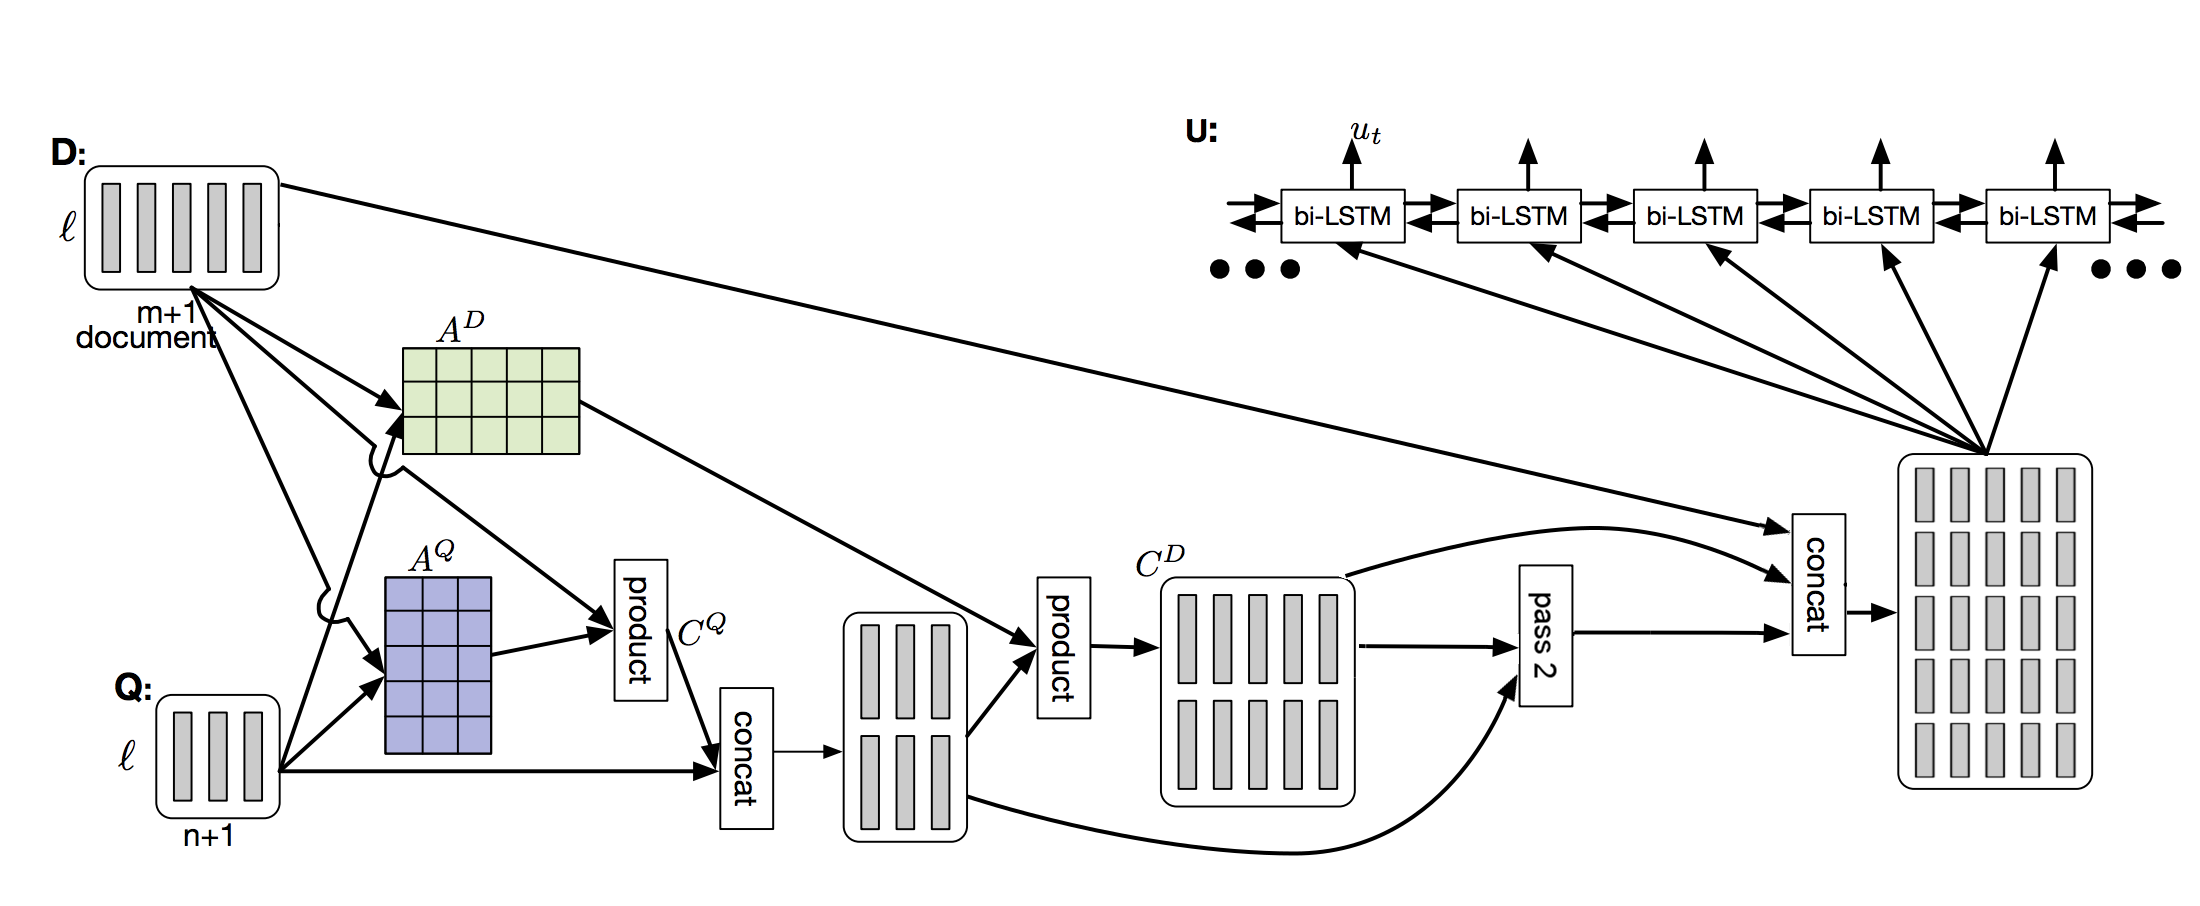
\includegraphics[width=0.9\textwidth]{images/coattn_encoder.png}
    \caption{The DCN Co-attention Encoder}
    \label{im:enc}
\end{figure}

\begin{figure*}[h]
    \centering
    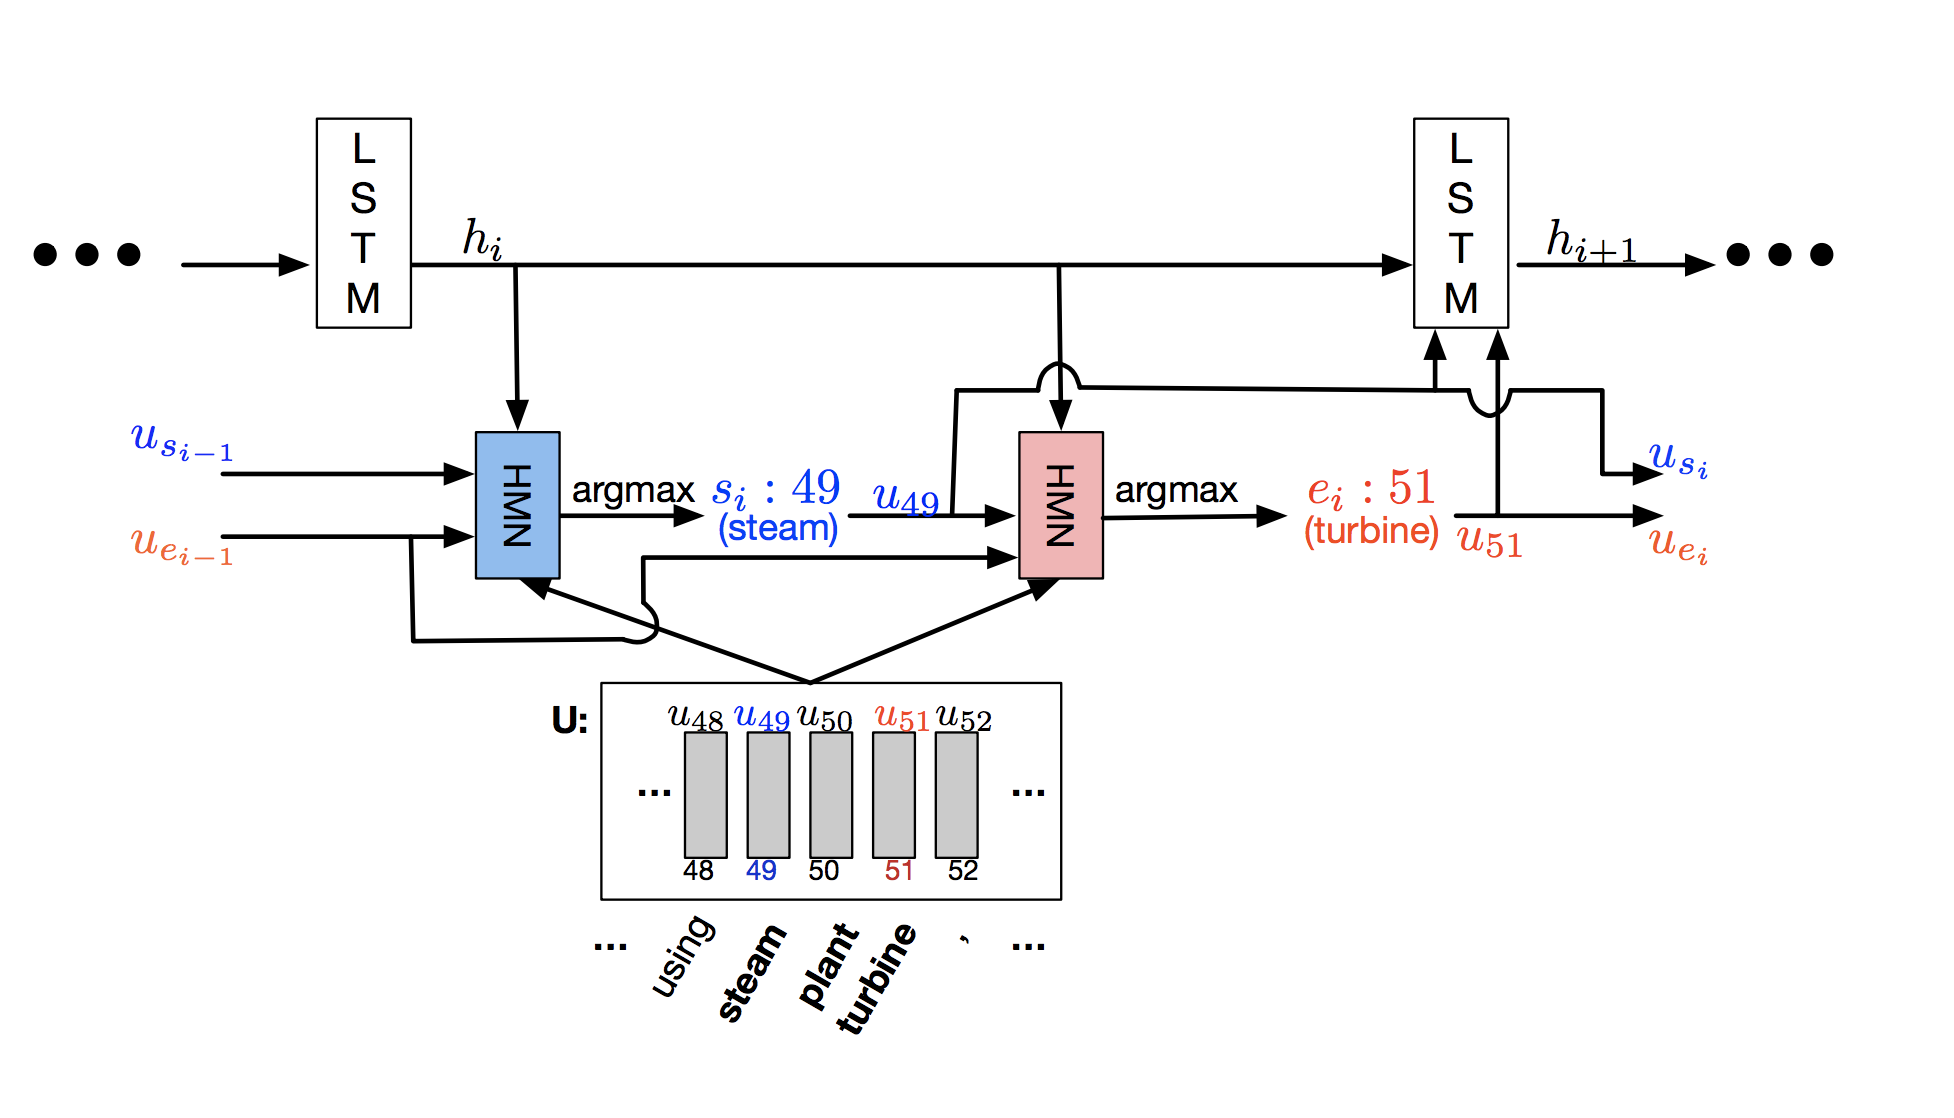
\includegraphics[width=0.85\textwidth]{images/decoder.png}
    \caption{The Dynamic Decoder Network}
    \label{im:dec}
\end{figure*}

\subsubsection{Experiments}

We first compute the GLoVe and CoVe word vectors for each word in the training and development data of the Stanford Question Answering Dataset (SQuAD) dataset, replacing all out of dictionary words with the zero vector. Then the network is trained with the Adam optimizer and the cross entropy loss for 40 epochs on a K80 GPU. A three-layer GRU network is used in the decoder network for all experiments, but we adjust the number of hidden units for the GRU networks that exist in the architecture. Experiments with 30, 100 and 200 hidden units per GRU are performed. An annealed learning rate initialized at 0.002 and a weight decay of 0.0001 is used during the training process. Gradient clipping is employed to prevent large gradients from destabilizing the training process, and early stopping is employed to stop training once overfitting is detected.

\subsection{Results on SQuAD}
The results on SQuAD with all the different variety of approaches we tried are presented in Table \ref{im:squad_res}. We present the results in a step by step fashion, showing how each of our modifications improves the results. We also note that we train our model for just 20 epochs compared to over 200 epochs used by the original model. Our best performing model qualifies to be ranked on the official SQuAD leader board.

\begin{figure*}[h]
    \centering
    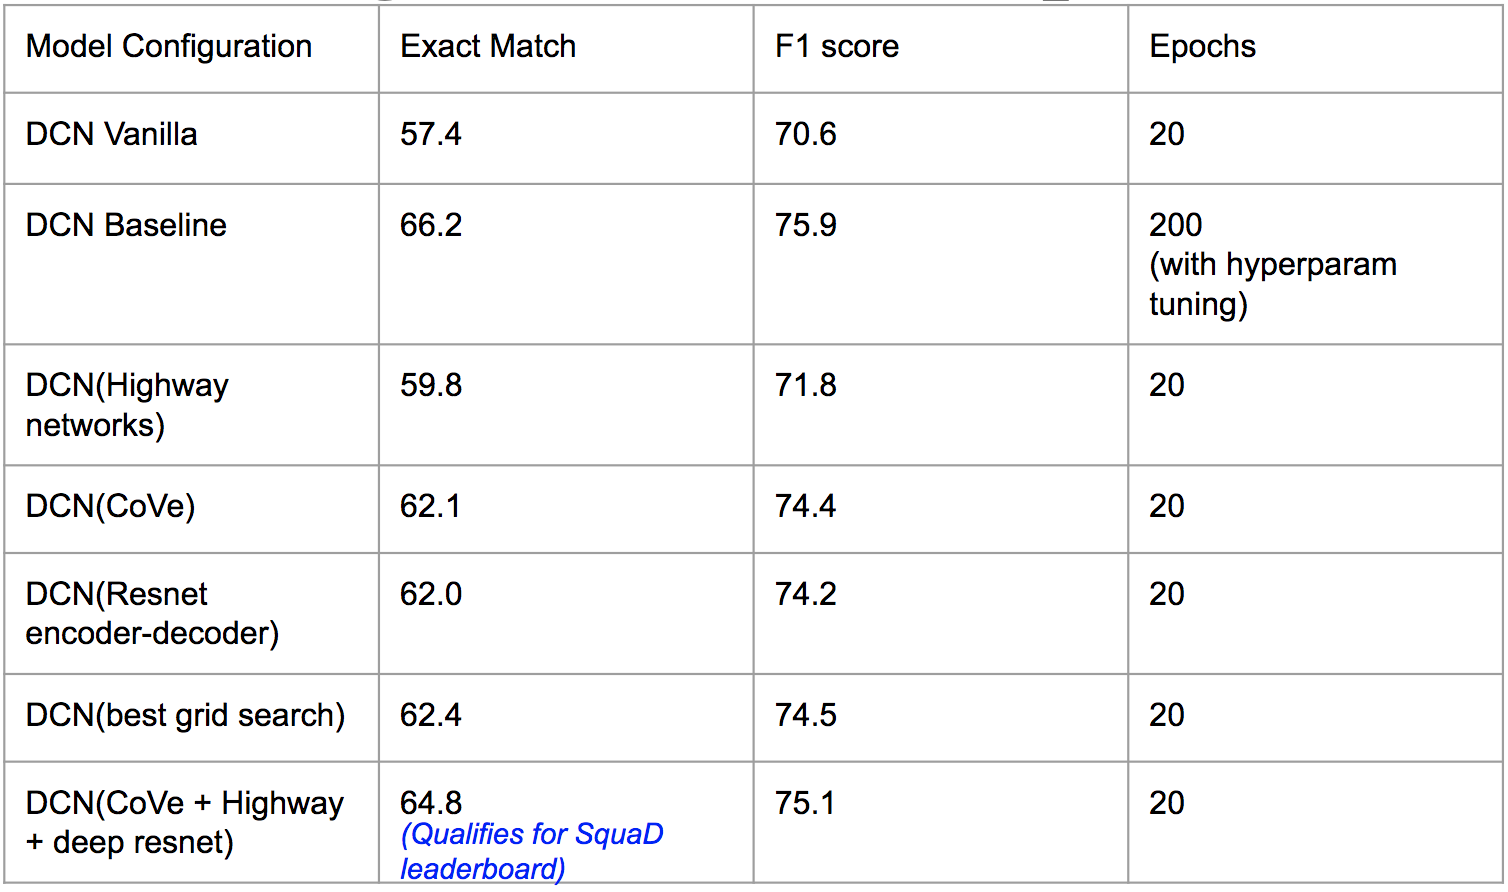
\includegraphics[width=0.85\textwidth]{images/res_squad.png}
    \caption{Results on the SQuAD dataset}
    \label{im:squad_res}
\end{figure*}

\begin{figure*}[h]
    \centering
    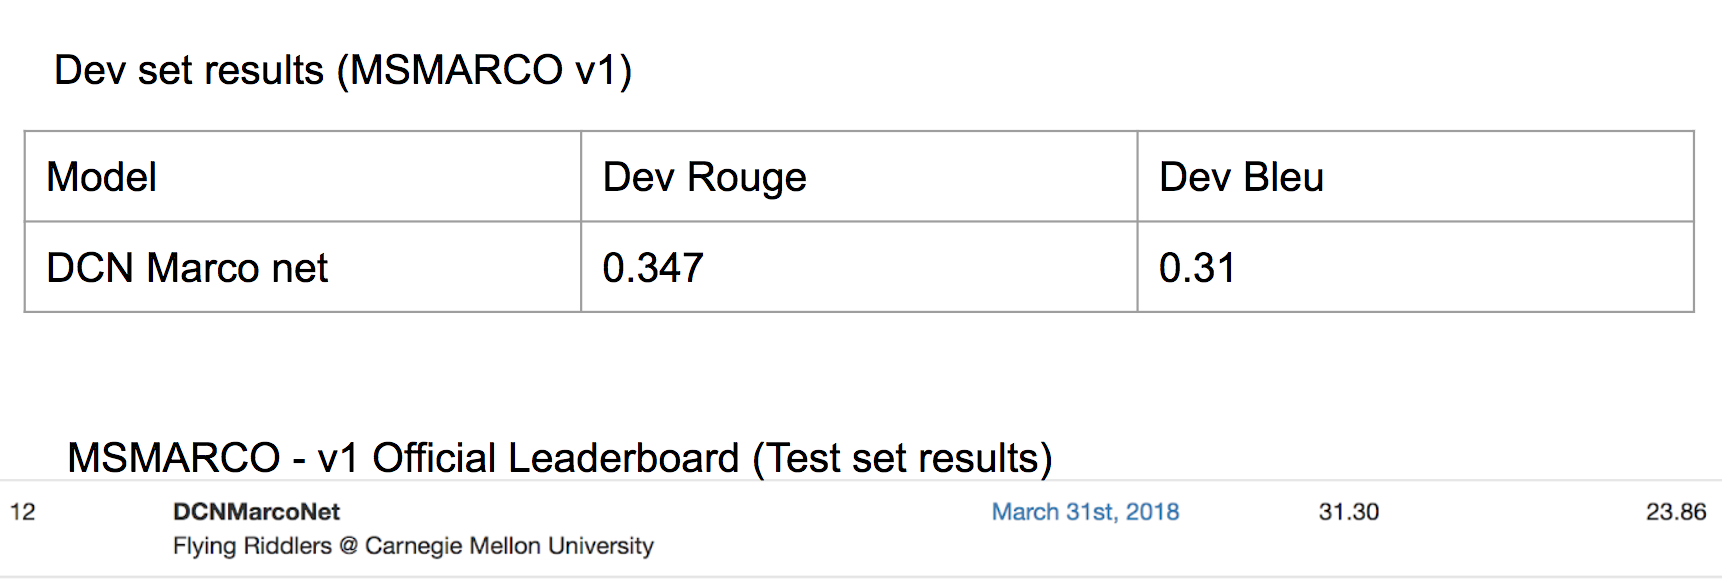
\includegraphics[width=0.85\textwidth]{images/res_marco.png}
    \caption{Results on the MSMarco v1 dataset}
    \label{im:res_marco}
\end{figure*}


An informal test is also performed with a small number of test cases not found in the data set. We find that the trained network has the capacity to answer these questions accurately as well. One out-of-dataset example is shown below:

\begin{table}
\begin{tabular}{|c|p{0.75\textwidth}|}
    \hline
    Document & The de Broglie–Bohm theory, also known as the pilot wave theory, Bohmian mechanics, Bohm's interpretation, and the causal interpretation, is an interpretation of quantum theory. In addition to a wavefunction on the space of all possible configurations, it also postulates an actual [...] The theory is named after Louis de Broglie (1892–1987) and David Bohm (1917–1992). \\
    \hline
    Question & After whom is pilot wave theory named after? \\
    \hline
    Predicted answer & Louis de Broglie \\
    \hline
\end{tabular}
\end{table}

This example demonstrates the ability of the network to resolve indirect relationships in the text, such as the chain connecting the phrase ``The theory [is named after]'' to its referent ``The de Broglie–Bohm theory'' to its alternative name ``the pilot wave theory''.

\subsection{Free Form Answer Generation}

Free Form answer generation is a relatively unexplored problem with little existing literature. Trying to solve this problem directly is a fairly hard task and would require an extremely complex network architecture which can not just look at huge text sources to detect the most relevant parts, but also compose a human like answer. This is too hard for most networks to achieve. To reduce the complexity of the problem being dealt by a single network, we use the spans predicted by our Dynamic Co-Attention Network as input to the Free Form answer generator network. This makes the network more powerful by giving it more information about the content of the expected answer and it now has to use this content information to compose an answer. \\

Natural Language generation is known to be one of the hardest problems on the NLP community due to the inability of modern day architectures to model long term context and generate syntactic and semantically coherent sentences. One of the primary issues we notice with such architecture is the ineffectiveness of the loss functions typically used in the seq2seq prediction networks typically used for this task. The seq2seq networks are usually based on LSTM encoder - decoder style architectures and typically penalize the generator using a cross entropy loss between the predicted and expected output word. Such work level loss metrics fail to capture global sentence level dynamics and completely miss out on enforcing syntactic and semantic coherence. We propose a novel loss metric here which we feel would be greatly useful in dealing with such issues.\\

First we introduce our generator network architecture. The architecture we propose is shown in Image \ref{im:im_gen}.
\begin{figure*}[h]
    \centering
    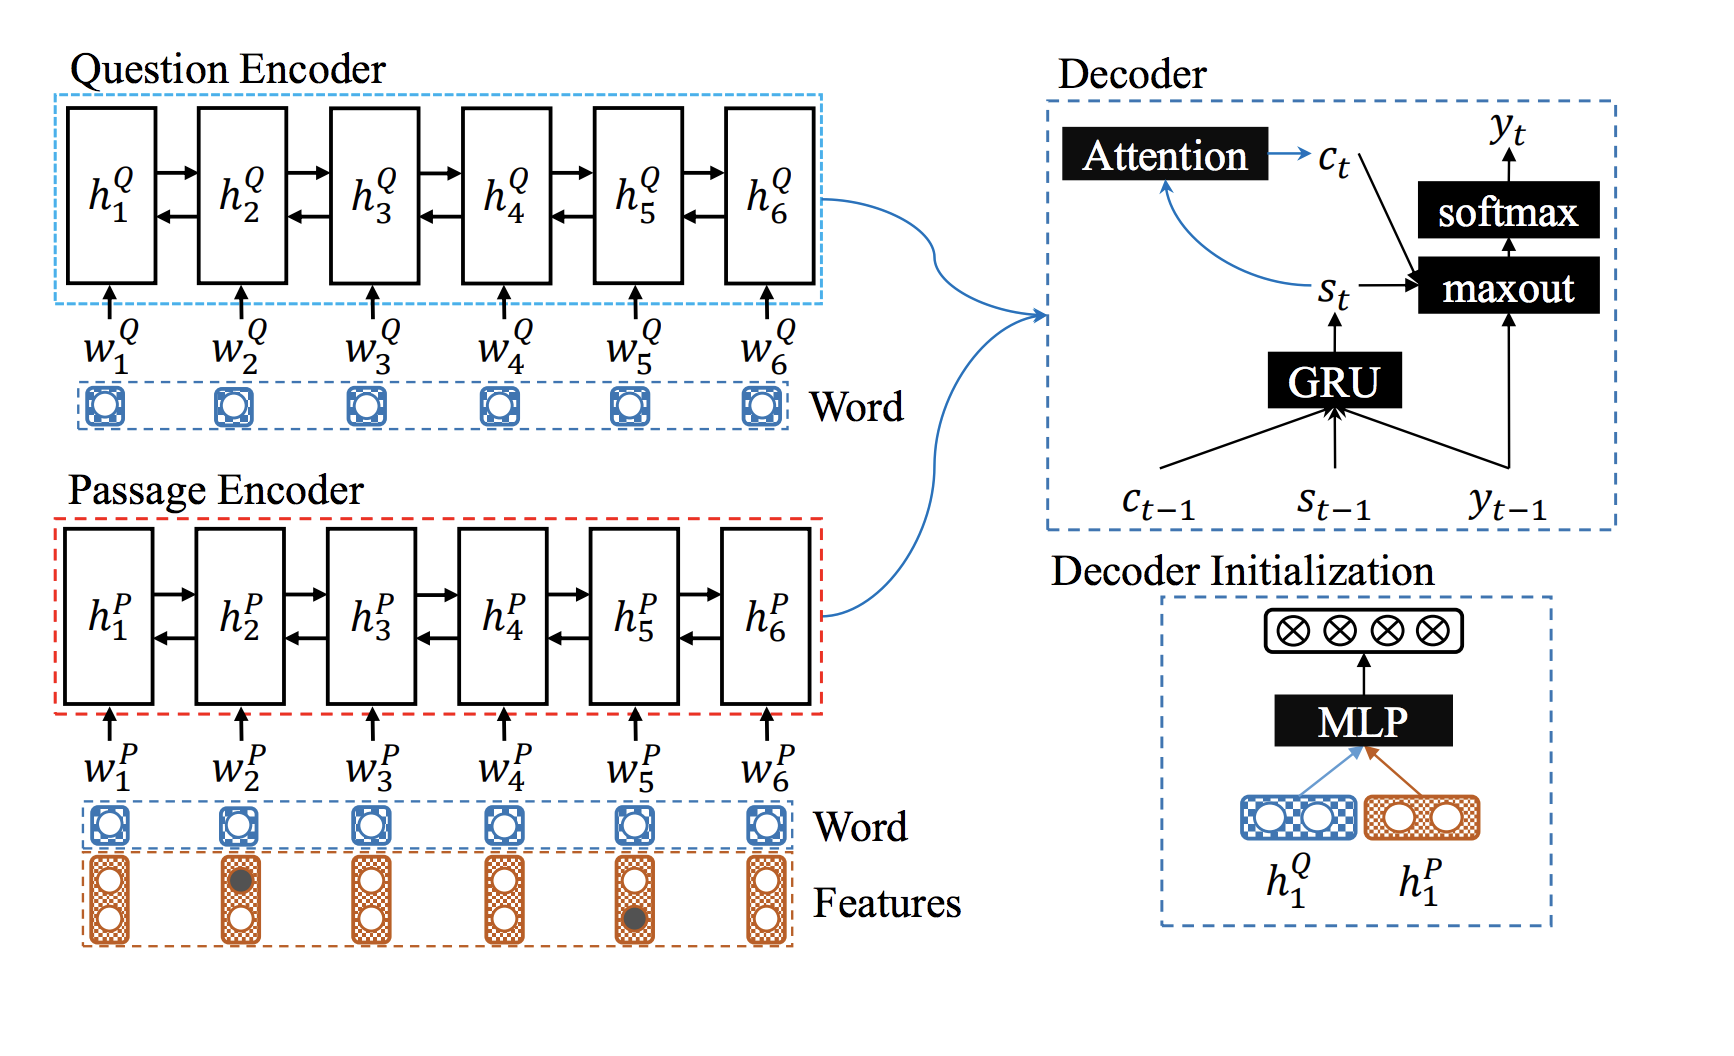
\includegraphics[width=0.85\textwidth]{images/ans_net.png}
    \caption{The Answer generator Network}
    \label{im:im_gen}
\end{figure*}

The network consists of a question encoder network, a paragraph encoder network and an attention based decoder network.\\
The question and passage encoder are Bidirectional GRU's which take as input the question and passage word embeddings, one word at a time and generate the respective question and passage embedding. This is given by the equations:

\[ {h_t}^P = BiGRU({h_{t-1}}^P, [{e_t}^P, {f_t}^e, {f_t}^e]) \]

\[{h_t}^Q = BiGRU({h_{t-1}}^Q, {e_t}^Q) \]

here ${h_t}^P$ and ${h_t}^Q$ denote the passage and question encoder hidden state at time t, ${e_t}^P$ and ${e_t}^Q$ denote the word embedding of  passage and question word at time t, ${f_t}^e$, ${f_t}^s$ are binary bits which are 0 or 1 depending of if the $t^{th}$ word in the passage is the start or end of a span i.e.  ${f_t}^e = 1$ if the $t^{th}$ word is the end of a span and 0 otherwise. Similarly ${f_t}^s = 1$ if the $t^{th}$ word is the start of the answer span and 0 otherwise.\\
The decoder is also a GRU which has a non linear combination of the question and passage encoding as its initial state denoted by:
\[ d_0 = tanh(W_d[{h_1}^P, {h_1}^Q] + b) \]
The rest of the decoder can be represented as:
\[d_t = GRU(w_{t-1}, {c^P}_{t-1}, {c^Q}_{t-1}, d_{t-1})\]
where $w_{t−1}$ is the word generated at the previous time step, $d_{t−1}$ is the previous decoder state and ${c^P}_{t-1}$ is the passage context vector which is learnt by computing the attention of the decoder state over the passage states. Similarly ${c^Q}_{t-1}$ is the context vector computed by taking the attention of the decoder state over the states of the question encoder. 

We experiment with two different types of attention mechanisms, which we call as the `additive attention mechanism' and the `dot attention mechanism'. \\
The additive attention mechanism is defined by the following equations.:\\
\[  {{s^P}_{t,j}} = {{v^P}_a}^Ttanh({W^P}_a(d_{t-1}) + {U_a}^P{h^P}_j )\]
\[{a^P}_{t,i} = softmax({{s^P}_{t,j}})\]
\[{c^P}_t = \sum_{i=1}^n {a^P}_{t,i} \cdot {h^P}_i\]

Similarly for question encodings:\\
\[  {{s^Q}_{t,j}} = {{v^Q}_a}^Ttanh({W^Q}_a(d_{t-1}) + {U_a}^Q{h^P}_j )\]
\[{a^Q}_{t,i} = softmax({{s^Q}_{t,j}})\]
\[{c^Q}_t = \sum_{i=1}^n {a^Q}_{t,i} \cdot {h^Q}_i\]

The dot attention on the other hand is defined by the equations:\\
\[  {{s^P}_{t,j}} = (d_{t-1})^T{h^P}_j \]
\[{a^P}_{t,i} = softmax({{s^P}_{t,j}})\]
\[{c^P}_t = \sum_{i=1}^n {a^P}_{t,i} \cdot {h^P}_i\]
Similarly for question encodings:\\
\[  {{s^P}_{t,j}} = (d_{t-1})^T{h^Q}_j \]
\[{a^P}_{t,i} = softmax({{s^P}_{t,j}})\]
\[{c^P}_t = \sum_{i=1}^n {a^P}_{t,i} \cdot {h^P}_i\]
These attention weighted question and passage encodings are fed to the decoder network.\\
To predict the next word we use the present decoder state, the question and passage context and the previous word and pass their combination through a Maxout layer, taking maxout over 2 successive units and then take a softmax over our vocabulary. This is represented by the equations:\\
\[r_t = W_rw_{t-1} + {U^P}_r{c^P}_t + {U^Q}_r{c^Q}_t + V_rd_t \]
\[m_t = [max{r_{t,2j-1}, r_{t,2j}}]^T \]
\[p(y_t|y_1, . . . , y_{t-1}) = softmax(W_o \cdot m_t) \]


\subsection{Results on MS MARCO}
We use our free form answer generation network on the MSMarco V1 dataset. The results for the same are listed in Image \ref{im:res_marco}. We note that we are listed as one of the highest ranked single model on the actual MSMarco leaderboard.

\subsection{Experiments and Results on BioASQ dataset}

We further extend our model to evaluate it on the BioASQ dataset. We use our DCN model to perform the QA task on the BioASQ dataset. Presently, we only work with factoid and list type of questions. The architecture is exactly the same as the DCN encoder. In place of the decoder we simply use the attention values over the passage to predict our answers. For both factoid and list type questions, the passage entities which attain attention more than a threshold are chosen as the correct answers. For the Factoid type answers, as the ranking of these entities also matters we return them in the order of decreasing attention weights. The results of this model evaluated on the BioASQ dataset after pre-training on the SQuAD dataset are presented in Table \ref{tab:bioasq_res}. Note that presently the model uses word2vec and Cove embeddings and hence several of the Biological entities are actually not a part of the vocabulary which may partially explain the poor performance of the DCN model on the BioASQ dataset.

\begin{table}
\begin{tabular}{|c|c|c|}
    \hline \hline
    Model & Factoid(MRR) & List(F1)\\
    \hline
    DCN MarcoNet& 0.11&0.07\\
    \hline \hline
\end{tabular}
    \caption{Results on the Bioasq dataset}
    \label{tab:bioasq_res}
\end{table}


\begin{table*}[h]
    \centering
    \begin{tabular}{|c|c|c|c|c|} 
    \hline \hline
    Model & Exact Answers & Exact Answers & Exact Answers & Ideal Answers \\
    &Yes/No type& Factoid  type& List type & All types \\
    & Accuracy (\%) & MRR & F1 score & ROUGE-2\\
    \hline \hline
    \cite{khyati-paper} & - & - & - & 0.653  \\
    \hline
    \cite{fudan}&\textbf{0.714}&0.272& 0.187& -\\
    \hline
    \cite{fastqa}& - &\textbf{0.392}& \textbf{0.361}&-\\
    \hline
    Sarrouti and Alaoui \shortcite{usmba}&0.461&0.207&0.243&0.577\\
    \hline
    \textit{BioAMA}(Ours)&0.653& 0.195&0.234&\textbf{0.721}\\
    \hline \hline
    
    \end{tabular}
    \caption{Comparison of our question-type based QA model with other state of the art approaches on BioASQ 5b dataset}
    \label{tab:comparison_results}
\end{table*}

\section{Discussion}

In this section, we shall analyze our gross findings from building the two QA systems and experimenting on both the datasets. Having built a broad set of classifiers and modules, we also comment on our experiences in building these systems while highlighting our key learning from these experiences. 

\subsection{Model Comparison}

The question-type based QA system that we built performs remarkably well on the BioASQ. This can be noted from the Table \ref{tab:comparison_results}, where we compare our system with the state of the art systems on BioASQ. We can see that our system performs the best on Ideal Answers and is very close to the best performances on Exact Answers. The trends are very similar for BioASQ 6b as well, indicating that a question-type based system is very effective for BioASQ. However, our end-to-end system fails to perform well on the BioASQ, as shown in Table \ref{tab:bioasq_res}, which leads us to the conclusion that for smaller datasets, a question-type based modular system is typically a much better choice of QA system.

On the other hand, we note that the end-to-end systems that we proposed has much better performances on the large datasets such as MS MARCO and SQuAD at the ranks of some of the state-of-the-art systems, while our modular question-type based system fails to yield to similar performance. This should not be surprising, since our end-to-end QA system is heavily parametrized and a lot more capable, and having a large dataset would help us efficiently train the model. In the cases of smaller datasets, however, we would have to aid the model with inductive biases, and constrain it with very few parameters to strike a trade off between efficient training and optimal performance. 

With these findings, we reject our general hypothesis that a holistic QA model can be trained to yield consistently high performances across multiple datasets, and conclude that a well performing QA system would have to be carefully chosen with the size and domain of the dataset as key considerations.

\subsection{Lessons Learned}

Building the two QA systems on two separate datasets involved a lot of design and implementation choices some of which, in hindsight, were sub-optimal. However, these have led us to have many insightful realizations, some of which are:

\begin{itemize}
    \item Yes/No questions have a stronger semantic component compared to many other question types
    \item Entailment-based tasks show high transfer learning potential
    Even simple linear transformation for embedding works well for augmenting word embeddings
    \item Since the yes/no answer is computed based on gross entailment statistics, the answers are less sensitive to errors in entailment
    \item An advantage of an unsupervised classifier is that class imbalances are handled well

\item Simple approaches can yield more reliable and strong results than complicated ones.
\item For small datasets, long and in-depth dataset exploration is the key point for feature engineering (statistical biases of the origin of the data).
\item However, it is important to not rely on specific aspects of a subset of the data. It’s easy to overfit if the features come from a bias of a subset.
\item Models for small datasets can be extremely sensitive of feature weighting and selection. 
\item Ranking (LeTor) approaches are strongly tied to computational power (after a certain point, pairwise is not realistic).

\item The most important features might seem very trivial but works very well ( Indri, BM25 etc.) 
\item Diversification plays an important role in removing redundancy in the summary generated
\item Inverse relation between word limit and Rouge
\item Dice coefficient works a tad bit better  with Indri as both are language model based.
\item If the answer is present in single snippet, narrowing down that snippet is hard (MS Marco) 
\item For Web search type queries, rules (PoS based) work surprisingly well as initial filter.
\item Summary of BioASQ and Description of MS Marco are not exactly the same. Summary is a subset of Description.

\end{itemize}

\section{Individual Contributions}

By virtue of having a tightly integrated system that was built collaboratively, we have had to work very closely with each other on almost all the modules involved. Though we all weighed in for the design and analysis of the systems, each one of us also assumed primary responsibility for implementation of specific parts of the system, which have been tabulated in Table \ref{tab:contributions}.

\begin{table}[h]
    \centering
    \begin{tabular}{c|c|c|c|c} \hline
    Team Member & Yes/No Type & Factoid/List Type & Ideal Answers & End-to-end System \\ \hline \hline
    Nitish & \checkmark & \checkmark & & \\
    Gabriel & & \checkmark & \checkmark & \\
    Pranavi & & \checkmark & \checkmark & \\
    Vasu & \checkmark & & & \checkmark \\ \hline
    \end{tabular}
    \caption{Key contributions from individual members of the team}
    \label{tab:contributions}
\end{table}

% Our key novel contributions in this paper are:
% \begin{enumerate}
%     \item \textbf{State of the art result on ideal answer questions}: Our proposed \textit{BioAMA} system attains state of the art results in automatic evaluation measures for the ideal answer questions in Task 5b of the BioASQ dataset, yielding a 7\%  improvement over the previous state of the art system \cite{khyati-paper}.
%     \item \textbf{Novel framework for Yes/No type QA}: 
%     We introduce a novel NLI-based approach for answering the Yes/No style questions in the BioASQ dataset. We model these questions as a Textual Entailment (TE) problem and use Hierarchical Convolutional Neural Network based Infersent models \cite{Infersent} to answer this type of question. To address the challenge of inadequate training data, we also introduce a novel embedding projection technique which allows for effective transfer learning from models trained on larger datasets with a different vocabulary to work on the much smaller BioASQ dataset.
%     \item \textbf{A novel two-stage approach to answer Factoid and List type questions}: 
%     By using an ensemble of biomedical NER taggers to generate a candidate answer set, we devise unsupervised and supervised ranking algorithms to generate the final predictions.
%     \item \textbf{Improved Maximum Marginal Relevance (MMR) framework}: We improve upon the MMR framework for relevant sentence selection from the chosen snippets. The use of MMR for sentence selection was introduced in the work of Chandu et al. \shortcite{khyati-paper}. We improve upon this framework by experimenting with a number of more informative similarity metrics to replace and improve upon the baseline Jaccard similarity metric.

% \end{enumerate}


\section{Conclusion and Future Work}
\label{future}
In this paper, we present a framework for tackling both ideal and exact answer type questions and obtain state of the art results on the ideal answer type questions on the BioASQ dataset. In our framework for ideal answers, we aimed at improving the Information Retrieval component of the extractive summarization. Although this improved ROUGE scores considerably, the human readability aspect of the generated summary answer is not improved to a great extent. We are presently working on using effective abstractive summarization based approaches like Pointer Generator Networks \cite{PGC} and Reinforcement Learning based abstractive summarization techniques \cite{salesforce} to try and improve the human readability aspect of our ideal answers. We aim to continue our research in this direction to adapt these networks to get a good balance between ROUGE score and human readability.



\bibliography{references}
\bibliographystyle{acm}

\appendix

\end{document}